\lab{Applications}{Image Segmentation}{Image Segmentation}

\objective{Understand some basic applications of eigenvalues to graph theory.}
\label{lab:ImgSeg_eigenvalues}

\section*{Graph Theory}
\begin{figure}

 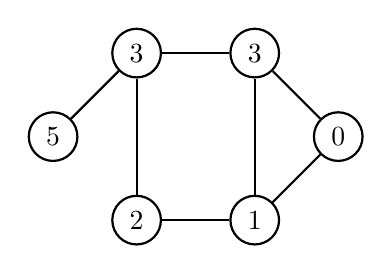
\begin{tikzpicture}[auto,node distance=1.5cm,
 thick,main node/.style={circle,draw}]

  \node[main node] (5) [] {5};
  \node[main node] (2) [below right of=5] {2};
  \node[main node] (3) [above right of=5] {3};
  \node[main node] (4) [right of=3] {3};
  \node[main node] (1) [right of=2] {1};
  \node[main node] (0) [below right of=4] {0};

  \foreach \s/\t in {5/3, 3/4, 4/0, 0/1, 1/2, 2/3, 1/4} {
   \path[draw] (\s) edge (\t);}
\end{tikzpicture}
\caption{A simple undirected graph}
\label{fig:example_graph}
\end{figure}

\begin{figure}
 \begin{tikzpicture}[->,>=stealth',shorten >=1pt,auto,node distance=1.5cm,
 thick,main node/.style={circle,draw}]

  \node[main node] (A) [] {A};
  \node[main node] (B) [below of=A] {B};
  \node[main node] (C) [right of=A] {C};
  \node[main node] (D) [below of=C] {D};
  \node[main node] (E) [right of=C] {E};
  \node[main node] (F) [right of=D] {F};

  \foreach \s/\t in {A/C, B/A, B/D, C/E, C/F, D/C} {
   \path[draw] (\s) edge (\t);}
\end{tikzpicture}
\caption{A simple directed graph}
\end{figure}



Graphs represent relationships between objects.
For example, the transition diagram in Figure \ref{fig:markov1} in Lab \ref{lab:EigSolve} shows the relationship between states in a Markov chain.
An undirected graph is a set of nodes (or vertices) and edges, where each edge connects exactly two nodes.

A graph is \emph{simple} if no edge connects a node to itself. 
The graph in Figure [TODO!] is simple, but the graph in Figure [TODO!] is not.

A \emph{weighted} graph is a graph with a weight attached to each edge.
For example, a weighted graph could represent a collection of cities with roads connecting them.
The vertices would be cities, the edges roads, and weight of an edge would be the length of a road.
Such a graph is depicted as in Figure [TODO!].

Any graph can be thought of as a weighted graph by assigning a weight of 1 to each edge.

\subsection*{Adjacency, degree, and Laplacian matrices}
We will now introduce three special matrices associated to a graph. 
Throughout this section, assume we are working with a weighted graph with $N$ nodes, and that $w_{ij}$ is the weight attached to the edge connecting node $i$ and node $j$.
We first define the adjacency matrix.

\begin{definition} The \emph{adjacency matrix} is an $N \times N$ matrix whose $(i,j)$-th entry is
\begin{center}
	$ \begin{cases}  w_{ij} & \mbox{if an edge connects node i and node j} \\ 0 & \mbox{otherwise.} \end{cases}$
\end{center}
%technically, the definition does not apply to all graphs (according to Wikipedia)
%however, this definition works if we are just considering simple graphs, i.e. at most one edge between any two vertices, no loops
\end{definition}

For example, the graph in Figure \ref{fig:example_graph} has the adjacency matrix
\[
\begin{pmatrix}
0 & 1 & 0 & 0 & 1 & 0\\
1 & 0 & 1 & 0 & 1 & 0\\
0 & 1 & 0 & 1 & 0 & 0\\
0 & 0 & 1 & 0 & 1 & 1\\
1 & 1 & 0 & 1 & 0 & 0\\
0 & 0 & 0 & 1 & 0 & 0
\end{pmatrix}.
\]
Notice that this adjacency matrix is symmetric. This will always be the case for undirected graphs.

\begin{comment}
Raising the adjacency matrix to a power yields some very interesting information.
We can discover the number of paths of length $n$ between two nodes by raising a graph's adjacency matrix to the $n$th power.
For example, by squaring $A$, we can find the number of paths of length two between every pair of nodes.
\begin{lstlisting}
>>> A = np.array([[0,1,0,0,1,0],[1,0,1,0,1,0],
                  [0,1,0,1,0,0],[0,0,1,0,1,1],
                  [1,1,0,1,0,0],[0,0,0,1,0,0]])

>>> np.linalg.matrix_power(A,2)
array([[2, 1, 1, 1, 1, 0],
       [1, 3, 0, 2, 1, 0],
       [1, 0, 2, 0, 2, 1],
       [1, 2, 0, 3, 0, 0],
       [1, 1, 2, 0, 3, 1],
       [0, 0, 1, 0, 1, 1]])
\end{lstlisting}
We can see that no paths of length two exist between node 0 and node 5 because $A^2_{0,5} = 0$.
By calculating $A^6$ we can find the number of paths of length six from node 3 to itself.
\begin{lstlisting}
>>> np.linalg.matrix_power(A, 6)
array([[45, 54, 38, 45, 54, 16],
       [54, 86, 29, 77, 51, 11],
       [38, 29, 55, 15, 70, 27],
       [45, 77, 15, 75, 31,  4],
       [54, 51, 70, 31, 93, 34],
       [16, 11, 27,  4, 34, 14]])
\end{lstlisting}
We see that there are 75 unique paths of length six from node 3 to itself.
Imagine trying to count all of those paths by hand!
It would be very easy to count incorrectly.
This method makes it very simple to count paths without mistakes.

Adjacency matrices can also be composed of \li{True} and \li{False} values.
In this case, the $n$th power of such a matrix (using boolean arithmetic)
is again a matrix of
boolean values which simply indicate whether there exists a path of length $n$ between the given pair of nodes, rather than indicating the number of such
paths.

\begin{problem}
Let the following matrix represent a directed graph
\[
\begin{pmatrix}
0 & 0 & 1 & 0 & 1 & 0 & 1 \\
1 & 0 & 0 & 0 & 0 & 1 & 0 \\
0 & 0 & 0 & 0 & 0 & 1 & 0 \\
1 & 0 & 0 & 0 & 1 & 0 & 0 \\
0 & 0 & 0 & 1 & 0 & 0 & 0 \\
0 & 0 & 1 & 0 & 0 & 0 & 1 \\
0 & 1 & 0 & 0 & 0 & 0 & 0
\end{pmatrix}
\]
Between which pair of nodes does there exist the greatest number of paths
of length five?
From which node to which node is there no path of length seven?
\end{problem}
\end{comment}

The second matrix is the degree matrix. 
\begin{definition} The \emph{degree matrix} is an $N \times N$ diagonal matrix whose $(i,i)$-th entry is
\[ 
\sum_{j=1}^N w_{ij}.
\]
This quantity is just the sum of the weight of each edge that touches node $i$.
\end{definition}
%For a directed graph, each node has an \emph{out-degree} (the number of edges directed away from a node) and an \emph{in-degree} (the number edges directed toward a node).
We call the $(i, i)-th$ entry of the degree matrix the \emph{degree} of node $i$.

Finally, we can combine the degree matrix and the adjacency matrix into the Laplacian matrix.
\begin{definition}
The \emph{Laplacian matrix} of a simple graph is 
\[D - A \]
where $D$ is the degree matrix and $A$ is the adjacency matrix of the graph.
\end{definition}


In this lab we will learn about graphs by studying their Laplacian matrices.
While the Laplacian matrix seems simple, we can learn surprising things from its eigenvalues.


\begin{problem}
Write a function that accepts the adjacency matrix of a graph as an argument. Use the adjacency matrix to check that the graph is undirected and has no self-edges. Then using the definition above, calcluate the Laplacian matrix.

Test your function by finding the Laplacian matrix of the graph in Figure \ref{fig:example_graph}. Your function should return the following Laplacian matrix:
\[
\begin{pmatrix}
2 &-1 & 0 & 0 &-1 & 0 \\
-1 & 3 &-1 & 0 &-1 & 0 \\
0 &-1 & 2 &-1 & 0 & 0 \\
0 & 0 &-1 & 3 &-1 &-1 \\
-1 &-1 & 0 &-1 & 3 & 0 \\
0 & 0 & 0 &-1 & 0 & 1 \\
\end{pmatrix}
\]
\label{prob:laplacian}
\end{problem}



\subsection*{Connectivity: first application of Laplacians}

A \emph{connected graph} is a graph where every vertex is connected to every other vertex by at least one path.
In applications, it is often important to know if a graph is connected.
What is the best way to find out?
A naive approachis to exhaustively search every possible path from each vertex.
While this works for very small graphs, most interesting graphs will have thousands of vertices (for example, the internet), and for such graphs this approach is not feasible.

Fortunately, there is a better way.
If the second smallest eigenvalue of its Laplacian matrix is positive, then a graph is connected. [TODO: cite something!]
In many applications the Laplacian matrix is sparse, so by taking advantage of this sparsity, we can cheaply determine if a graph is connected.

\begin{problem}Write a function \li{laplacian} that accepts an adjacency matrix as an argument and returns the Laplacian matrix and its second smallest eigenvalue.
Use the \li{scipy.linalg} package to compute the eigenvalue.

Use \li{numpy.random.rand(n,n)} to generate two random matrices of sizes n=10 and n=100.
Then use masking to change the sparsity of each of the matrices, i.e. \li{numpy.random.rand(n,n) > c} for \li{c = 0.25,0.95}. This will create four different matrices of boolean values. Remember that when doing calculations with boolean values that \li{True} is considered to be a 1 and \li{False} is considered to be a 0. Is the n=10 adjacency matrix connected when we let c=.25? What about when we let c=.95? Is the n=100 adjacency matrix connected when c=.95?
\end{problem}


\section*{Image Segmentation: second application of Laplacians}

\begin{figure}
    \centering
    \begin{subfigure}{0.31\textwidth}
        \includegraphics[width=\textwidth]{RegMon.png}
    \end{subfigure}
   \hspace*{\fill}
    \begin{subfigure}{0.31\textwidth}
        \includegraphics[width=\textwidth]{NegMon.png}
    \end{subfigure}
    \hspace*{\fill}
    \begin{subfigure}{0.31\textwidth}
        \includegraphics[width=\textwidth]{PosMon.png}
    \end{subfigure}
    
\caption{An image and its segments.}
\label{fig:monument}
\end{figure}
Image segmentation is the process of finding natural boundaries in an image (see for example Figure \ref{fig:monument}).
This is an easy task for humans, who can easily pick out portions of an image that ``belong together.''
In this lab, you will learn one way to program a computer to segment images.

The algorithm we will present comes from a paper by Jianbo Shi and Jitendra Malik in 2000. [TODO cite; how does this relate to the other paper]
Their idea is to represent an image as a weighted graph as follows. 
To a computer, an \emph{image} is a collection of \emph{pixels}. 
Each pixel has a brightness and coordinates describing its location in the image.
To define a graph representing this image, we let every pixel be a vertex.
Two pixels are connected if the distance between their coordinates is small (less than $r$).
The weight of the edge connecting two pixels is related their similarity in brightness, where a low weight means they are very different.

After defining this graph, we will segment the image by ``cutting'' (or removing) edges with low weights, which represent lines of high contrast in the image. 
The ``cut'' is the total weight of the edges removed. Thus, to segment an image, we wish to minimize the ``cut.''

Now let us define the adjacency matrix of the graph associated to an image. 
Since an $N \times N$ image has $N^2$ pixels, the adjacency matrix will be $N^2 \times N^2$.
After choosing a radius $r$ and some constants $\sigma_I$ and $\sigma_d$, we define the adjacency matrix to be $W = (w_{ij})$, where

\begin{equation}
\label{eq:adjacency}
w_{ij} = \begin{cases} \exp(-\frac{|I(i) - I(j)|}{\sigma_I^2}-\frac{d(i,j)}{\sigma_d^2}) & \mbox{ for $d(i,j) < r$} \\ 0 & \mbox{ otherwise,} \end{cases}
\end{equation}
where
\begin{itemize}
	\item$d(i,j)$ is the Euclidean distance between pixel $i$ and pixel $j$
	\item $|I(i) - I(j)|$ is the difference in brightness of pixels $i$ and $j$.
\end{itemize}

Notice that $W$ will be sparse as long as $r$ is small.

\subsection*{Computing the adjacency matrix}

In the following problem we will write a function that finds the adjacency matrix of an image, based on the definition from \eqref{eq:adjacency}. To do this, we first flatten the image we are working on. 

\begin{lstlisting}
nodes = img.flatten()
\end{lstlisting}

This allows us to index all of the pixels (or nodes) using a one-dimensional array. By doing this, we are better able to calculate the weights in-between pixels. It is important to note here that this is only one way of indexing the pixels in our image. We can still index the pixels in our image or matrix by using standard tuple notation. So for example, given a $2 \times 2$ matrix we can access the bottom-right element (if we are starting at row 0 and column 0) by the tuple (1,1). If we choose to flatten our matrix we can index the same element by the number 3 (if we once again start at 0).

Since each pixel is only connected to the pixels within radius $r$, relatively few entries of our adjacency matrix will be non-zero. For this reason, we will work with sparse matrices from the \li{scipiy.sparse} package. We first initialize our adjacency matrix as a sparse matrix.

\begin{lstlisting}
W = spar.lil_matrix((nodes.size, nodes.size), dtype=float)
\end{lstlisting}
We use \li{lil_matrix} because it gives us an efficent way to build our matrix piece by piece. To learn more about sparse matrices in scipy read the documentation at \url{http://docs.scipy.org/doc/scipy/reference/sparse.html}.

At this point we can initialize the main diagonal of the degree matrix. We only care about the main diagonal because the degree matrix is a diagonal matrix.
\begin{lstlisting}
D = np.zeros((1, nodes.size))
\end{lstlisting}
Now we go through each pixel of our image matrix to calculate the weights.

\begin{lstlisting}
# 'height' is the original height of the image
# 'width' is the original width of the image
for row in xrange(height):
    for col in xrange(width):
        # Calculate the index of the pixel at (row, col) relative to the
        # flattened array 'nodes'. 
        rowcol = row * width + col
\end{lstlisting}
Say we start with pixel \li{A}. Notice that we do not need to find the weights between every pixel and pixel \li{A}, since most of the weights will be 0. We only need to find the weights between pixel \li{A} and those pixels that are within radius $r$ of pixel \li{A}. 

A helper function has been provided that finds the pixels and corresponding distances within radius $r$ of a single pixel. Note that the pixel being passed into the function is indexed as a tuple, or more precisely as a given row and column index. The function returns however, an array of indices in the flat array form (single numbers) of pixels within radius $r$ of the pixel passed into the function.
\lstinputlisting[style=fromfile]{getNeighbors.py}
Below we use the helper function to get the indices and distances.

\begin{lstlisting}
# find the indices and distances of the pixels that are within 
# distance r of the current pixel by calling getNeighbors
indices, distances = getNeighbors(row, col, radius, height, width)
\end{lstlisting}
We can then calcluate the weights between pixels by using definition \eqref{eq:adjacency}. The helper function already calculates the distances, so now we just need to find the difference in brightness of pixels by subtracting the corresponding pixels.
Once we find the weights we can then add them into our adjacency matrix. 
\begin{lstlisting}
# 'weights' is the weights between the pixel we are on and the pixels within
# radius r
W[rowcol, indices] = weights
\end{lstlisting}
We can also calculate part of the main diagonal of the degree matrix.
\begin{lstlisting}
D[0,rowcol] = weights.sum()
\end{lstlisting}
We now loop to the next pixel and repeat the process.

After we have found our adjacency matrix (\li{W} in the code we have provided above) we convert it to a \li{csc} format, and return both \li{W} and \li{D}. 
\begin{lstlisting}
W = W.tocsc()
return W, D
\end{lstlisting}
The sparse matrix format \li{csc} is better for computations which we will want to use later.




\begin{problem}
Write a function \li{adjacency} that takes an $N \times N$ image array, radius $r$, and values for
$\sigma_I^2$ and $\sigma_d^2$, and returns the adjacency matrix defined in \eqref{eq:adjacency}. Test your function on the image \li{dream.png}. This image is read in as a color photo so first convert it to grayscale to reduce it to two dimensions.
\begin{lstlisting}
# read in the image
img_color = plt.imread('dream.png')
# convert to grayscale
img = (img_color[:,:,0]+img_color[:,:,1]+img_color[:,:,2])/3.0
\end{lstlisting}
Let $r=5.0$, $\sigma_I^2=0.02$ and $\sigma_d^2=3.0$.


%Notice that for each pixel you can save time by only checking the pixels $r$ rows and columns away.
%For that you'll have to handle the pixels on the edges and corners of the image carefully.
%I gave them new helper code, which abstracts away the edge cases.
\label{prob:adjacency_dream}
\end{problem}

\subsection*{Minimizing the 'cut'}

As was mentioned before, we are trying to minimize the `cut', or the total weight of the edges we remove to create segments. This problem comes down to finding the second smallest eigenvalue of $D^{-1/2}QD^{-1/2}$, where $D$ is the degree matrix and $Q$ is the Laplacian matrix of the adjacency matrix defined in \eqref{eq:adjacency}. The mathematics behind this is quite involved, so the reader is encouraged to read the paper that Shi and Malik wrote at \url{http://www.cs.berkeley.edu/~malik/papers/SM-ncut.pdf} for a better understanding.
	
To calculate $D^{-1/2}QD^{-1/2}$, we once again use sparse matrices. We use the \li{adjacency} function from Problem \ref{prob:adjacency_dream} to find the adjacency matrix \li{W} and the main diagonal of the degree matrix \li{D}. We can convert \li{D} into a diagonal sparse matrix using \li{spar.spdiags}.

\begin{lstlisting}
Ds = spar.spdiags(D, 0, D.shape[1], D.shape[1], format = 'csc')
\end{lstlisting}

In like manner we can find the diagonal sparse matrix $D^{-1/2}$. We can also calculate the Laplacian matrix $Q$ since \li{Ds} and \li{W} are both sparse matrices and in `csc' format. To matrix multiply two sparse matrices together, use the \li{dot} function. For example, if \li{M} and \li{N} are two sparse matrices, use \li{M.dot(N)}.

The eigenvector associated with the second smallest eigenvalue will be a $N^2 \times 1$ vector and will have positive and negative entries. If we reshape this vector to be the same size as our original image we can create a mask that will create two segments - one segment corresponding to the positive values of the eigenvector and the other segment corresponding to the negative values of the eigenvector. 

\begin{lstlisting}
# create a mask array that is True wherever the eigenvector is positive.
# reshape it to be the size of img.
mask = (eigvec>0).reshape(img.shape)
\end{lstlisting}
To find the segments, we only need to take the product of our mask with the original image.

\begin{lstlisting}
# create the positive segment by masking out the pixels in img 
# belonging to the negative segment.
pos = img*mask
\end{lstlisting}
By recursively executing this function, we can find segments within segments.


\begin{problem}  Write a function \li{segment} that solves the segmentation problem for small images.
Accept an image array as an argument and return the two segments.
Use $r = 5.0, \sigma_I^2 = 0.02,$ and $\sigma_d^2 = 3.0$.
Remember that the Laplacian matrix will be very large, but also very sparse.
Because of the way we defined $\sigma_I^2$ the image matrix intensity values need to be between $0.0$ and $1.0$. If this is not standard for the images you are using, change $\sigma_I^2$.

Test your function on the image \li{dream.png}. Your segments should look like the segments in Figure \ref{fig:dream_solution} with the original image on the left.
\end{problem}

\begin{figure}
\centering
    \centering
    \begin{subfigure}{0.31\textwidth}
        \includegraphics[width=\textwidth]{RegDream.png}
    \end{subfigure}
    \hspace*{\fill}
    \begin{subfigure}{0.31\textwidth}
        \includegraphics[width=\textwidth]{NegDream.png}
    \end{subfigure}
    \hspace*{\fill}
    \begin{subfigure}{0.31\textwidth}
        \includegraphics[width=\textwidth]{PosDream.png}
    \end{subfigure}
\caption{Segments of \li{dream.png}}
\label{fig:dream_solution}
\end{figure}